\chapter{Prozess}

\section{Allgemein}

\subsection{Arbeitsdokumentation} 

Ich hatte jeden Tag ein Heft in meiner Schultasche mit mir getragen, in welchem ich auftauchende Ideen sofort notierte.
Wenn ich dann wieder an meinem Computer sass, wurden diese Ideen nochmals durchgeschaut und entweder verworfen oder implementiert.
Ich sorgte dafür, dass ich jede Woche \textbf{mindestens einmal} daran arbeitete, und hörte, wenn ich mal begonnen hatte, auch nicht so schnell wieder auf.
In einer Textdatei \lstinline{journal/quellen.txt} führte ich ein Arbeitsjournal in welchem ich festhielt, wann ich woran gearbeitet habe.
Die Versionskontrolle erfolgte über \textbf{GitHub}. Damit bin ich abgesichert für den Fall, dass Daten verloren oder kaputt gehen würden. Auch wenn ich beim Entwickeln feststelle, dass die Version von vor zwei Tagen besser funktionierte als die jetzige, kann ich auf diese zurück wechseln.
Der Entwicklungsfortschritt wird mit Git automatisch erfasst.

\subsection{Inspirationsquellen}
Was das Erfinden der Objekte und Geschichte angeht, diente mir vor allem meine rege Fantasie als Inspiration.
Doch ab und an half auch diese nichts, gerade wenn es um komplizierte Funktionalitäten ging (z.B. Sicht-Vektoren für Interaktionen und der Sprung des Spielers).

In diesen Fällen konsultierte ich eine Webseite namens Udemy. Diese bietet eine grosse Spannweite an Kursen. Mein Vater hatte mir dort vor ein paar Monaten einen Programmierkurs für C\# geschenkt, welcher sich nun als nützlich erweisen sollte.
Dieser Kurs war eine auf sich aufbauende Videoserie, in welcher ein 2D Spiel von A-Z entwickelt wurde.
Da mein Spiel jedoch 3D sein sollte und der Udemy Kurs beim besten Willen nicht alle Thematiken abdecken konnte, blieb mir als oft letzte Hoffnung noch die öffentliche Tutorialwebseite und das Forum von Unity. \footfullcite{unity3dtutorial}


\subsection{Vorgehen}
Nachdem ich die grundlegenden Objekte wie den Spieler und die einfachen Funktionen wie z.B. Laufen erstellt hatte, ging es daran, das Spiel zu erweitern. Ich bin nicht einer der wenigen, die sich ein Skript im Kopf überlegen und dies dann fehlerfrei beim ersten Versuch zum laufen kriegen können, noch nicht. Wenn es also an die Umsetzung einer Idee ging, schrieb ich den Code in ein schon existierendes Skript.
Falls es nicht funktionierte, wurde entweder ein anderer Ansatz gewählt oder ich arbeitete daran bis es geklappt hat.

Sobald funktional alles glatt lief, musste der Code aufgeräumt werden. Dabei wurden die noch vorhandenen Spuren der nicht erfolgreichen Versuche entfernt, der gewünschte Code allenfalls bereinigt und vereinfacht. Das Aufräumen oder Auslagern passierte entweder dadurch, dass ich den Code manuell geändert bzw. den getesteten Code in ein neues Skript hinein kopierte, oder indem ich den Code mit Hilfe von MonoDevelop umgebaut habe.

\subsection{Code-Umbau}
\label{subsubsec:refactoring}
Das Umbauen von Code ist vor allem in der objektorientierten Programmierung sehr wichtig, was dem Vorgang seinen eigenen Namen einbrachte: Refactoring. Ins deutsche wurde es als \glqq Refaktorisieren\grqq übersetzt, was eigentlich falsch ist, da das umbauen von Code wenig mit  dem Faktorisieren der Mathematik zu tun hat.
Treffender wäre der Begriff \glqq Restrukturierung\grqq.


\paragraph{Umbennen}\mbox{} \\
Wenn ich einfach vorwärts arbeite, leidet meine Rechtschreibung sehr stark. Ebenfalls tendiere ich dazu, während dem Kommentieren in andere Sprachen zu fallen. Ich habe auch während des Kodierens manchmal die Gross- und Kleinschreibung nicht eingehalten. Standard ist aber, alle Methoden Gross anfangen, Variablen und Eigenschaften hingegen klein.

Beim Umbenennen wird also folgendes gemacht:
Wenn ich nun ein rein textuelles "Suchen und Ersetzen" machen würde, könnte es passieren, dass an gewissen Stellen etwas falsch ersetzt wird und dann könnte nicht mehr kompiliert werden.
Um dies zu beheben hat MonoDevelop einen eigenen Mechanismus, welcher NUR genau die angegebene Variable/Methode/Eigenschaft verändert, und diese überall.

Das einzige, was manuell angepasst werden muss, ist der Dateiname des Skripts beim Umbenennen der Hauptklasse (Hauptklasse und Dateiname müssen übereinstimmen) und deren Referenzen in der Unity Umgebung.

\paragraph{Vereinfachen}\mbox{} \\
Beim Entwickeln kann es passieren, dass mehrmals hintereinander die gleichen Aufrufs-Ketten stehen. Aus Gründern der Lesbarkeit und Geschwindigkeit ist es sinnvoll, diese in eine Variabel zwischenzuspeichern. Dabei unterstützt einen die Monodevelop IDE:

\begin{figure}[H]
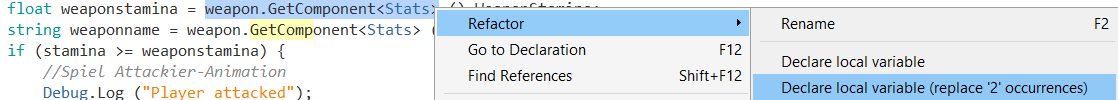
\includegraphics[scale=0.67]{screenshots/refactor.png}
\caption{Vereinfachen des GetComponent<> Aufrufs}
\end{figure}

Das Resultat schaut folgendermassen aus:

\begin{lstlisting}[caption={Code nach Vereinfachung}]
var stats = weapon.GetComponent<Stats> ();
float weaponstamina = stats.WeaponStamina;
string weaponname = stats.WeaponName;
\end{lstlisting}

\paragraph{Aufteilen}\mbox{} \\
Wenn es grosse Code-Teile waren, die neu entstanden, dann sollten die benötigten Teile eigenständig werden, denn ein einziges riesiges Skript welches das ganze Spiel steuert ist weder besonders gut für das rasche Arbeiten, noch wird es von anderen Programmierern/Programmiererinnen gerne gesehen, da die Übersichtlichkeit verloren geht.
Während dem Entwickeln des Waffenwechsels im Playerskript wurde der Code immer grösser. Nach einer Zeit ergab es Sinn, diesen Teil des Codes in ein eigenes Skript auszulagern, nicht zuletzt zur besseren Übersichtlichkeit.

\section{Problemstellungen und deren Umsetzung}

\subsection{Spielführung}
Damit das Spiel wirklich gut benutzbar wird, benötigt es gewisse Funktionen, die den Spieler unterstützen und an der Hand durch das Spiel begleiten:
\begin{itemize}
\item Um nicht jedes Mal neu anfangen zu müssen, gibt es ein Menü mit der Möglichkeit des Unterbruchs und Wiederaufnahme des Spiels, verbunden mit einer Speicherfunktion des Spielstands.
\item Das Head-Up-Display (HUD) hat die Aufgabe, dem Spieler alle nötigen Informationen über den Zustand seiner Spielfigur zu liefern.
\end{itemize}

\subsubsection{Start Menü}
Skript: Menu.cs\\\\
Das Menü beinhaltet vier Elemente: Einen \textbf{Canvas}, also eine Art \glqq Plache\grqq, die für uns hier als Hintergrundabdunklung fungiert. Dann gibt es 3 Buttons:

\begin{figure}[H]
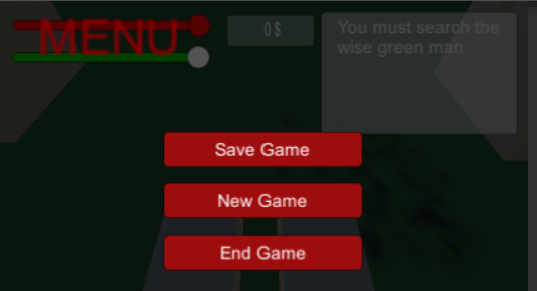
\includegraphics[scale=1]{screenshots/menuscreen.png}
\caption{Menü}
\end{figure}


\paragraph{New Game}
Dies setzt alle gespeicherten Spieldaten zurück und startet das Spiel neu.

\begin{lstlisting}[caption={New Game}]
// Startet ein neues Spiel
public void OnButtonNewPressed ()
{
	print ("Write some code here");
	player.gameData.InitNewGame ();
}

\end{lstlisting}

\paragraph{Save Game}
Dieser Knopf bewirkt, dass bestimmte Daten wie die X-, Y-, Z-Position des Spielers, Gegners sowie wichtige Spieldaten wie Gesundheitszustand etc. in eine Datei geschrieben werden. Bei einem Neustart des Spiels werden diese Angaben wieder eingelesen und übernommen.

\begin{lstlisting}[caption={Save Game}]
// Speicherfunktion
public void OnButtonSavePressed ()
{
	Debug.Log ("Speichern");
	player.gameData.SaveGame ();
}
	
\end{lstlisting}

\paragraph{End Game}
Das Knopf führt einen Unity Befehl namens \lstinline{Application.quit}  aus, welcher das ganze Programm beendet. 

\begin{lstlisting}[caption={End Game}]
// Beendet das Spiel
public void OnButtonEndPressed ()
{
	Debug.Log ("Spiel Beendet");
	Application.Quit ();
}
\end{lstlisting}

\subsubsection{GameData}
Skript: GameData.cs\\\\
Um die Daten des aktuellen Spiels zu speichern oder diejenigen des letzten Spiels zu laden, schuf ich die Klasse GameData.
Mit Hilfe der PlayerPref Klasse schreibt oder liest sie übergebene Daten in oder aus eine/r Datei. 
Im Folgenden zeige ich die fürs Speichern verwendete Reihe von Aufrufen.
\begin{lstlisting}[caption={Methode zur Speicherung des Spielstandes in GameData}]
public void SaveGame ()
{
	PlayerPrefs.SetInt ("GameState", 0);
	player.SaveState (this);
	(...)
}
\end{lstlisting}


\begin{lstlisting}[caption={Methode SaveState in Player}]
	public void SaveState (GameData gameData)
	{
		gameData.SaveTransform ("player", transform);
	}
\end{lstlisting}

\begin{lstlisting}[caption={Methode SaveTransform in GameData}]
	public void SaveTransform (string scope, Transform transform)
	{
		Vector3 position = transform.position;

		PlayerPrefs.SetFloat (scope + "X", position.x);
		PlayerPrefs.SetFloat (scope + "Y", position.y);
		PlayerPrefs.SetFloat (scope + "Z", position.z);
	}
\end{lstlisting}

\subsubsection{Head-Up-Display (HUD)}
Skript: HUD.cs\\\\
Ein Head-up-Display ist eine Anzeigefläche, die sich nicht aus dem Sichtfeld bewegt, auch wenn der Benutzer seinen Kopf neigt und oder schwenkt.
Somit sind die Informationen in jeder Situation ablesbar.

\begin{figure}[H]
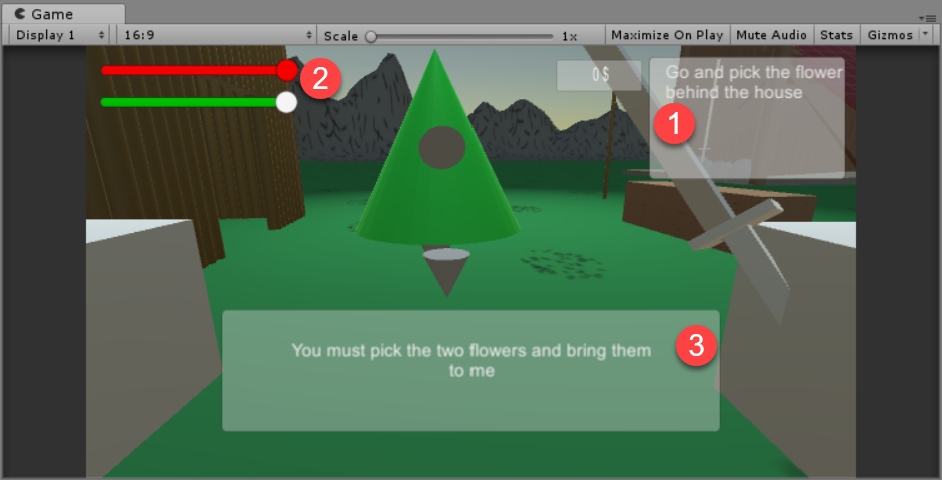
\includegraphics[scale=0.8]{screenshots/hud.png}
\caption{HUD}
\end{figure}

 
\paragraph{Aufgabenbereich (1)}\mbox{} \\
Der Aufgabenbereich befindet sich oben rechts.
Darin wird die jeweils aktuelle Aufgabe angezeigt.

\paragraph{Zustandsdisplay (2)}\mbox{} \\
Das Zustandsdisplay befindet sich oben links im HUD.
Es besteht aus zwei Schiebereglern \lstinline{Slider}, einem für die Gesundheit \lstinline{player.health} und einem für die Ausdauer \lstinline{player.stamina} des Spielers.
Ein Schieberegler ist ein 2D Balken, der einen Wert verkörpert. Man kann ihm in der Entwicklungsumgebung einen minimalen und einen maximalen Wert geben. Hier ist das bei beiden 0-100:

\begin{figure}[H]
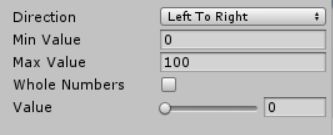
\includegraphics[scale=1]{screenshots/nullhundert.png}
\caption{Schieberegler Konfiguration}
\end{figure}

\noindent Abgefüllt werden diese Balken durch das HUD-Skript, welches bei jedem \lstinline{Update} Aufruf die aktuellen Werte aus dem \lstinline{Player} ausliest und an die Schieberegler weitergibt.

\begin{lstlisting}[caption={Schieberegler aktualisieren}]
public class HUD : MonoBehaviour
{
	(...)
	// Gesundheit Schieberegler
	private Slider healthSlider;
	// Ausdauer Schieberegler
	private Slider staminaSlider;
	(...)
	// Statusinformationen aus Spieler übernehmen und anzeigen
	void Update()
	{
		(...)
		healthSlider.value = player.health;
		staminaSlider.value = player.stamina;
		(...)
	}
}
\end{lstlisting}

\paragraph{Kommunikationsbereich (3)}\mbox{} \\
Der Kommunikationsbereich befindet sich im unteren Drittel des Bildschirmes.
Normalerweise ist er deaktiviert und damit unsichtbar.
Aktiviert wird er dann, wenn eine Methode, z.B. ein \lstinline{Interact}, das Attribut \lstinline{lastTalk} des Players neu setzt. 

\begin{lstlisting}[caption={Kommunikation setzen}]
void Interact(Player p)
{
	(...)
	p.lastTalk = "You must pick the two flowers ...";
	(...)
}
\end{lstlisting}

Dann erscheint eine Sprechblase mit dem entsprechenden Text. Im folgenden Codeausschnitt wird gezeigt, wie das Ein- und Ausschalten der Sprechblase und  das Aktualisieren des beinhalteten Textes funktioniert. Dies geschieht in der periodisch aufgerufenen \lstinline{Update} Methode, zum besseren Verständnis: \lstinline{Time.time} liefert die Zeit in Sekunden seit Spielstart.

\begin{lstlisting}[caption={Sprechblase ein- und ausblenden}]
public class HUD : MonoBehaviour
{
	// Die Spielerinstanz, welche alle Informationen liefert
	public Player player;

	// Feld, welches die Sprechblase beinhaltet
	private GameObject talking;
	// Textobjekt, welches den gesprochenem Text anzeigt
	private Text talkingText;
	// Zeitpunkt, als die letzte Blase angezeigt wurde, 0 wenn keine 
	// angezeigt wird
	private int speechDisplayedTime = 0;
	// Darstellungszeit der Sprechblase
	private const int speechDisplayDuration = 15;

	(...)
	
	// Update wird pro frame einmal aufgerufen
	// Statusinformationen aus Spieler übernehmen und anzeigen
	void Update()
	{
		(...)
		string lastTalk = player.lastTalk;
		// wenn mit dem Spieler seit letztem Mal gesprochen wurde
		if (lastTalk.Length > 0) {
			// anzeigen der Sprechblase
			player.lastTalk = "";
			talking.SetActive(true);//hier wird die Sprechblase aktiviert
			talkingText.text = lastTalk;
			// Zeitpunkt des Anzeigens merken
			speechDisplayedTime = (int)Time.time;
		} else {
			// kein neuer Text, überprüfe ob die Sprechblase 
			// wieder versteckt werden soll
			if (speechDisplayedTime > 0) {
				if ((int)Time.time - speechDisplayedTime > 
					speechDisplayDuration) {
					speechDisplayedTime = 0;
					talking.SetActive(false);//hier wird die Sprechblase deaktiviert
					talkingText.text = "";
				}
			}
		}	
	}
}
\end{lstlisting}

\subsection{Spieler}

Das 3D Modell des Spielers besteht rein aus Würfeln und Rechtecken:

\begin{figure}[H]
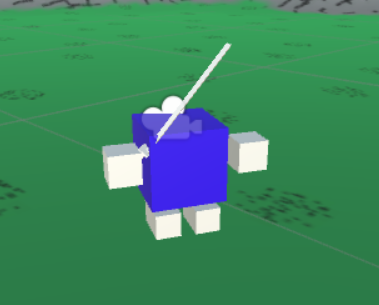
\includegraphics[scale=1]{screenshots/player.png}
\caption{Player 3D Modell}
\end{figure}

Die Funktionalität für den Spieler ist auf verschiedene Klassen verteilt:

\subsubsection{Player}
Skript: Player.cs\\\\
In dieser Klasse finden sich die Funktionen für den Zustand des Spielers (z.B. Gesundheit und Ausdauer), die Fortbewegung und die Interaktionen mit anderen Objekten.

\paragraph{Gesundheitszustand}\mbox{} \\
Der Gesundheitszustand wird im HUD angezeigt und kann über einen Methodenaufruf z.B. von Waffen verändert werden.
Der Player wie auch der NPC haben beide in ihrem eigenen Script das Setup ihrer Gesundheit.
\begin{lstlisting}[caption={Gesundheit als öffentliche Variable}]
// Gesundheit
public float health = 100f;
\end{lstlisting}
Um die Gesundheit zu verändern benutze ich eine Methode, in welcher der Wert um den die Gesundheit geändert werden soll in den Aufruf mitgegeben wird. Dieser kann sowohl positiv als auch negativ sein.
Er wird dann zur vorherigen Gesundheit addiert.

Dass die Gesundheit nicht über 100 geht und falls sie unter 0 geht, man auch tatsächlich stirbt, dafür sorgen die If-statements. Für den NPC sieht es so gut wie gleich aus:
\begin{lstlisting}
public void ChangeHealth(float change)
{
	health += change;

	if (health > 100.0f)
		health = 100.0f;
	else if (health < 0.0f) {
		Debug.Log("YOU ARE DEAD");
		model.SetActive(false);//lässt das gameObject verschwinden
	}
}
\end{lstlisting}
Wichtig ist, dass alle Veränderungen über diese Methode gemacht werden, damit es nur \textbf{einen Ort} gibt, an welchem Entscheide über Tod gefällt werden können.

\paragraph{Laufen}\mbox{} \\
Der hier gezeigte Codeausschnitt beinhaltet das Abfragen der Bewegungsinputs und deren Umsetzung.
Danach wird die Laufanimation initialisiert.

\begin{lstlisting}[caption={Laufen}]
	// x und z Koordinaten Bewegung
	float x = Input.GetAxis ("Horizontal") * Time.deltaTime * speed;
	float z = Input.GetAxis ("Vertical") * Time.deltaTime * speed;
        
	// Animationen
	anim.SetFloat ("forward", z * 3);
	anim.SetBool ("Walking", true);
	(...)
	transform.Translate (x, 0, z);
\end{lstlisting}

\paragraph{Springen}\mbox{} \\
Um zu springen muss der Spieler zuerst noch den Boden berühren.
Ob sich etwas unter ihm befindet, wird mit einem \lstinline{Raycast} überprüft, einem virtuellen Strahl.
Wenn dieser Raycast etwas trifft, ist Springen erlaubt.
Der Sprung erfolgt, indem ich dem Spieler eine Anfangsgeschwindigkeit in Y-Richtung (=Kraftstoss aus der Physik) gebe. Den Rest übernimmt Unitys Physik-Komponente.

\begin{lstlisting}[caption={Springen}]
	// raycast für "isgrounded"
	RaycastHit hit;
	(...)
	if (Input.GetAxis ("Jump") > 0f) {
		// isgrounded: Vektor Richtung Boden mit Länge 1. 
		// Wenn er etwas trifft, ist isgrounded true (was bedeutet,
		// dass springen möglich ist). Wenn nicht, dann nicht. 

		if (Physics.Raycast (transform.position, Vector3.down, out hit, 1)) {
			Debug.DrawLine (transform.position, hit.point);
			print (hit.distance);
			Vector3 power = rigid.velocity;
			power.y = 5f;
			rigid.velocity = power;
		}
	}
\end{lstlisting}

\paragraph{Kämpfen}\mbox{} \\
Beim Angriff wird im \lstinline{Player} zunächst überprüft, ob überhaupt noch genügend Kraft für den Einsatz der individuellen Waffe vorhanden ist. Wenn ja, dann wird sie verwendet und die Ausdauer des Players um den Betrag vermindert.

\begin{lstlisting}[caption={Angriff}]
	// Angriff
	if (Input.GetButtonDown ("Fire1")) {	
		// hole und vergleiche Waffenwerte
		GameObject weapon = GetComponent<WeaponManager> ().getActiveWeapon();
		var stats = weapon.GetComponent<Stats> ();
		float weaponstamina = stats.WeaponStamina;
		string weaponname = stats.WeaponName;
		if (stamina >= weaponstamina) {
			// Spiel Attackier-Animation
			Debug.Log ("Player attacked");
			if (weaponname == "Katana" || weaponname == "Bo")
				anim.Play ("Katana 0");
			else if (weaponname == "Hands")
				anim.Play ("Katana 0"); 
			ChangeStamina (-weaponstamina);
		}
	}
\end{lstlisting}
		
Die weiteren Abläufe beim Kämpfen des Spielers werden im \cref{subsec:weapons} beschrieben.

\subsubsection{Drehbewegung des Spielers}
Skript: MouseLookAtIt.cs\\\\
Im Gegensatz zu allen anderen Code-Ausschnitten die mit einer Art Bewegung zu tun haben geht es hier nicht um eine Verschiebung, sondern um eine Drehung.
Dieser Code sorgt dafür, dass sich für eine Links/Rechts Drehung die Spielfigur selbst bewegt, für eine Auf/Ab Bewegung hingegen nur die Kamera (Kopf).


\begin{lstlisting}[caption={Drehbewegungen}]
	// Ermittle die Maus-Position
	rotationY += Input.GetAxis ("Mouse X") * sensitivityY;
	rotationX += Input.GetAxis ("Mouse Y") * sensitivityX;
	rotationX = Mathf.Clamp (rotationX, minimumX, maximumX);
	rotationY = Mathf.Clamp (rotationY, minimumY, maximumY);
	
	// Bewege das Gameobject für die Links-/Rechts-Bewegung
	transform.localEulerAngles = new Vector3 (0, rotationY, 0);
	// und die Kamera für die Auf-/Ab-Bewegung
	cam.transform.localEulerAngles = new Vector3 (-rotationX, 0, 0);
\end{lstlisting}

\subsection{Animationen}
In Unity Animationen zu erstellen braucht etwas Geschick und viel Geduld. Jede der drei Spezies hat drei Animationen.

\subsubsection{Die verschiedenen Animationen}
\paragraph{Lauf-Animation}

Die Lauf-Animation besteht daraus, dass der Fuss gehoben nach vorne geht und gesenkt nach hinten. Diese Animation wird versetzt auf den zweiten Fuss kopiert, so dass immer, wenn der eine Fuss hinten ist, der andere vorne ist und umgekehrt. Die grösste Schwierigkeit bei dieser Animation war es, die beiden Füsse auf einander abzustimmen. Dazu kam, dass die Fortbewegungsgeschwindigkeit des Objekts ungefähr mit der Fussbewegung der Animation übereinstimmen sollte. TheThirdKind hat zwar eine Laufanimation, benutzt sie jedoch aktuell nicht, da er sich noch nicht bewegt.

\paragraph{Untätig-Animation}
Die Untätig-Animation (oder auch \textbf{Idle-Animation}) war die einfachste Animation zum Erstellen, da sie rein aus einem synchronen heben und senken der Hände besteht.

\paragraph{Angriffs-Animation}

Diese Animation war die schwierigste, da sie neben einer Positionsveränderung auch eine Drehung verlangte.
Das Problem war, dass bei einer Drehung der Hand diese aus ihrer Form fiel und die in der Hand gehaltene Waffe ebenso falsch skaliert wurde.
Dieses Problem behob ich mit Feintuning an den Kurven.
Das bedeutet es verändert sich immer noch ein wenig, aber nicht mehr in einem störenden Ausmass.

\subsubsection{Erstellen einer Animation}
Um eine Animation neu hinzuzufügen gibt man ihr zuerst einen Namen.
Danach öffnet sich ein leeres Fenster des Unity-Animators \footfullcite{unity3danimationeditor}
.
Dort hinein kann man per drag and drop GameObjekte hinzufügen und wählen, ob man Rotation, Proportion oder Position verändern will (es gibt noch viele andere Optionen, die man verändern 
kann, aber diese habe ich nicht benutzt).

\begin{figure}[H]
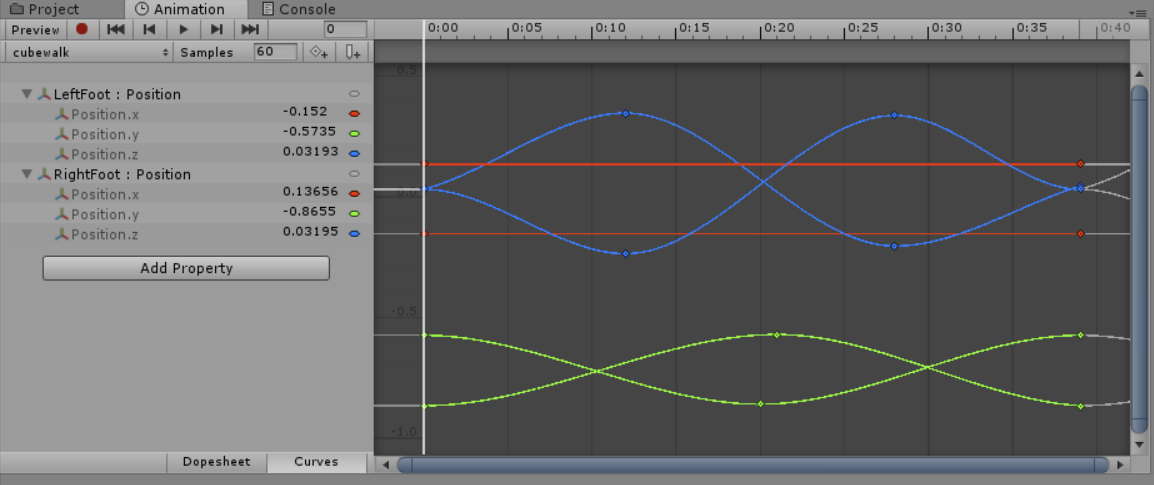
\includegraphics[scale=0.7]{screenshots/animations.png}
\caption{Animationskurven}
\end{figure}

In diesem Beispiel handelt sich hier um eine Laufanimation, welche nur die Füsse kontrolliert. Links sieht man die einzelnen Elemente mit ihren X-, Y- und Z-Koordinaten mit dazugehöriger Farbe. Rechts sind die Kurven, welche beschreiben, wie sich diese Koordinaten im Ablauf der Animation verändern (zum Beispiel hier sichtbar: Bewegung nur in Y und Z Koordinaten, die X-Koordinate bleibt unverändert (rot)).
Man sieht hier besonders, wie sich die Füsse nicht ruckartig, sondern fliessend und einander entgegengesetzt bewegen.

\subsubsection{Animator}
Der Animator ist das Element, welches den Wechsel zwischen verschiedenen Animationszuständen steuert. Zeiger können von einem Zustand auf einen anderen verweisen. Diese Übergänge kann man wiederum an Bedingungen koppeln.
\begin{figure}[H]
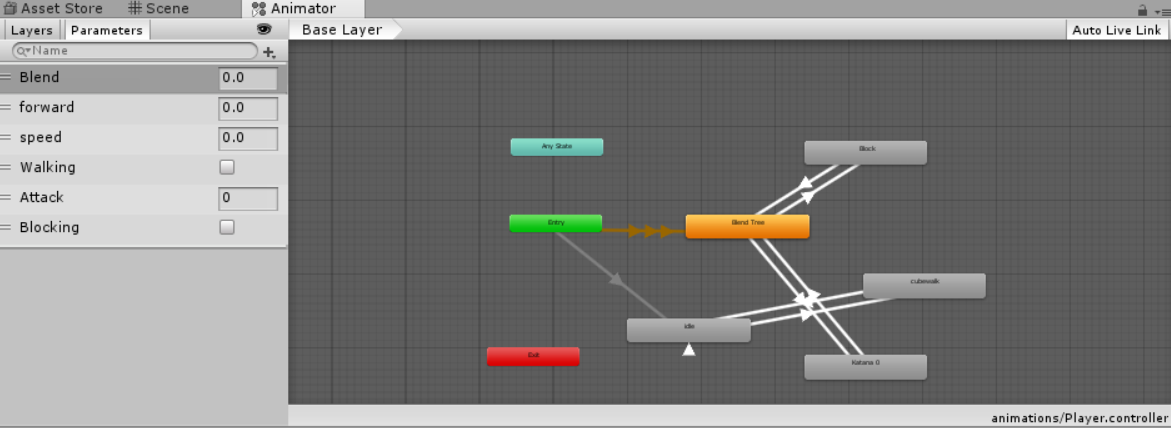
\includegraphics[scale=0.67]{screenshots/animator.png}
\caption{Animator mit Zuständen und deren Übergängen}
\end{figure}

\subsection{Waffen}
\label{subsec:weapons}
%todo shuriken?

Es gibt drei  Waffen: Das Katana, das Bo, und die Fäuste.
Jede Waffe hat verschiedene Werte was Schaden, Ausdauerkosten und Reichweite angeht.
\begin{figure}[H]
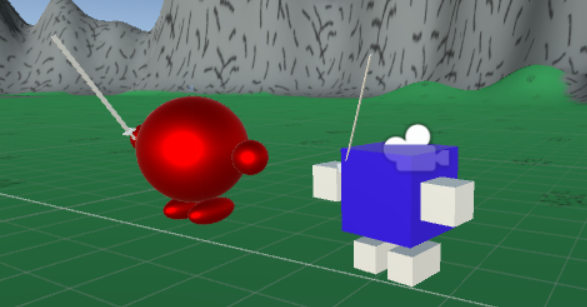
\includegraphics[scale=1]{screenshots/katana.png}
\caption{Katana}
\end{figure}

\begin{figure}[H]
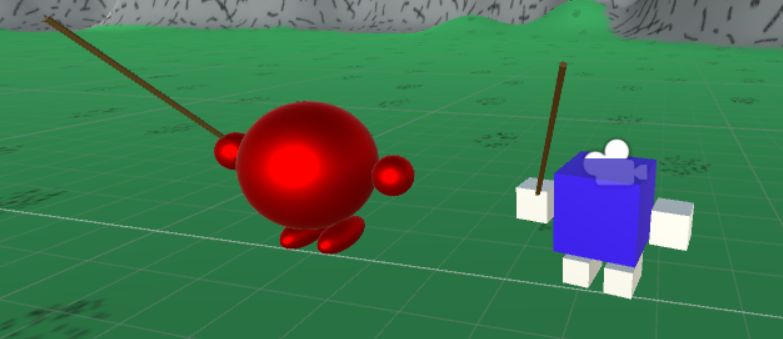
\includegraphics[scale=1]{screenshots/bo.png}
\caption{Bo}
\end{figure}



\subsubsection{Stats}
Skript: Stats.cs\\\\
Diese Klasse führt die Werte der Waffen. Die jeweiligen Werte werden in der Programmierumgebung deklariert. Diese verwenden dann die anderen Klassen.

\begin{lstlisting}
public string WeaponName = "Katana";
public float WeaponDamage = 35;
public float WeaponDefense = 15;
public float WeaponRange =	3;
public float WeaponSpeed = 3;
public float WeaponStamina = 10;
\end{lstlisting}

\begin{figure}[H]
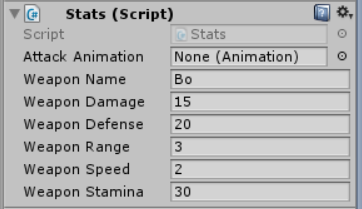
\includegraphics[scale=1]{screenshots/bostats.png}
\caption{Bo Stats Werte}
\end{figure}

\subsubsection{WeaponHit}
Skript: WeaponHit.cs\\\\
Jede Waffe hat einen \lstinline{Collider} (siehe \cref{subsubsec:collider}). Dieses Element löst ein \lstinline{OnTriggerEnter} Ereignis aus, sobald es mit einem anderen \lstinline{Collider} in Berührung kommt.
Das hier verwendete Script ermittelt das Kennzeichen des getroffenen Objekts und fügt Schaden zu, entweder dem Gegner oder dem Spieler selbst, je nachdem ob es sich dabei um ein Element mit dem Tag "Enemy" oder mit dem Namen "Player" handelt. %todo fix "enemy"
Der Wert des Schadens berechnet sich aus der Waffenwirkung, welche es aus den \lstinline{Stats} der jeweiligen Waffe ausliest. Dieser wird dann dem getroffenen Objekt zugefügt.

\begin{lstlisting}[caption={Waffentreffer}]
damage = Self.GetComponent<Stats>().WeaponDamage;

void OnTriggerEnter(Collider col)
{
	if (col.tag == "Enemy") {
		GameObject.Find (col.name).GetComponent<NPC>().ChangeHealth(-damage);
		Debug.Log(damage + " Damage applied to " + col.name);
	} else if (col.name == "Player") {
		GameObject.Find (col.name).GetComponent<Player>().ChangeHealth(-damage);
		Debug.Log(damage + " Damage applied to " + col.name);
	}
}
\end{lstlisting}

\subsubsection{WeaponManager.cs}
Skript: WeaponManager.cs\\\\
Der WeaponManager verwaltet die verschiedenen Waffen und wird verwendet, um die aktive Waffe zu wechseln \footfullcite{forumweaponsswitching}.

\begin{lstlisting}[caption={Wechsel der Waffen ja nach Taste}]
	void Update ()
	{
		// Wechseln der Waffe
		if (isplayer == true) {
			if (Input.GetAxis ("1") > 0f) {
				SetActiveWeapon (Katana);
				equipped = "Katana";
			}

			if (Input.GetAxis ("2") > 0f) {
				SetActiveWeapon (Bo);
				equipped = "Bo";
			}

			if (Input.GetAxis ("3") > 0f) {
				SetActiveWeapon (Hands);
				equipped = "Hands";
			}
		}
	}
\end{lstlisting}

\begin{lstlisting}[caption={Aktivieren einer Waffe}]
	private void SetActiveWeapon (GameObject activeWeapon)
	{
		for (int j = 0; j < weaponList.Count; j++) {
			if (weaponList [j] == activeWeapon) {
				for (int i = 0; i < enabledWeaponList.Count; i++) {
					if (enabledWeaponList [i] == activeWeapon) {
						weaponList [j].SetActive (true);
						weaponInHand = activeWeapon;
					}
				}
			} else {
				weaponList [j].SetActive (false);
			}
		}
	}
\end{lstlisting}

Die Methode \lstinline{SetActiveWeapon} hat die Aufgabe die \lstinline{activeWeapon} zu aktivieren und alle anderen zu deaktivieren, sonst würden sie gleichzeitig erscheinen.

\subsection{Figuren}

\subsubsection{InteractibleObject}
\label{subsubsec:interactibleobject}
Skript: InteractibleObject.cs\\\\
Alle GameObjekte mit denen interagiert werden kann sind von dieser Klasse oder erben von dieser.
Die Funktion \textbf{Interact} sendet einen Strahl vom Spieler aus. In der Entwicklungsumgebung kann dies während des Spiels dargestellt werden (1).

\begin{figure}[H]
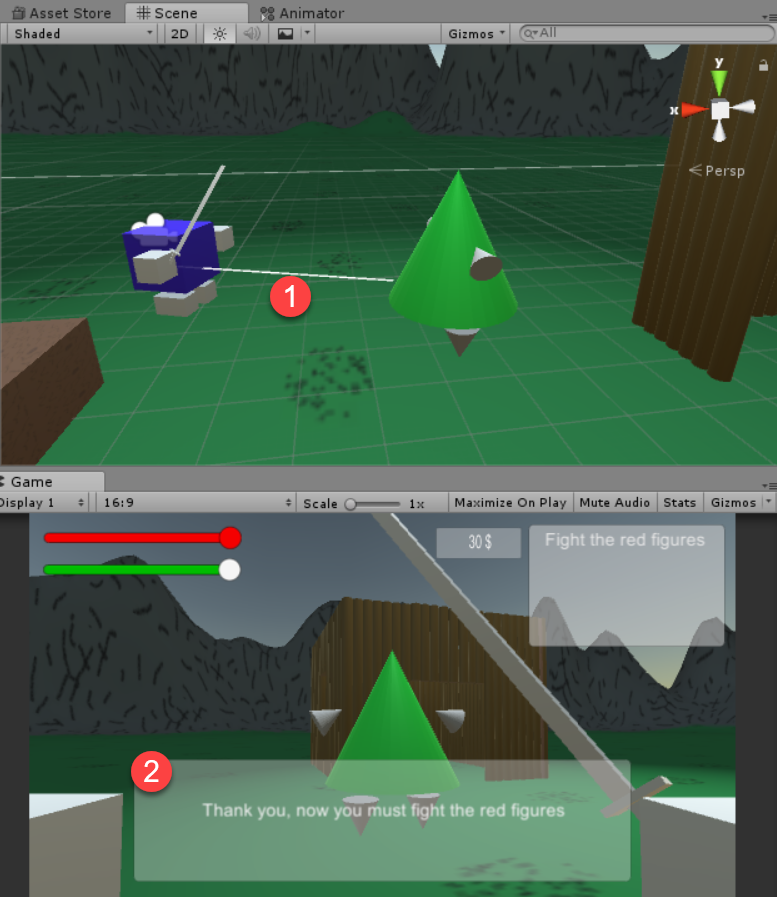
\includegraphics[scale=0.5]{screenshots/raycastthirdkind.png}
\caption{Vektorabfrage bei Interaktion mit \lstinline{TheThirdKind}}
\end{figure}

Wenn dieser Strahl etwas trifft wird überprüft, ob das getroffene GameObject den Tag \textbf{Interactive} hat. Falls ja, wird eine Nachricht \lstinline{Interact} an das getroffene Objekt geschickt. Falls der Tag nicht vorhanden ist, passiert nichts.

\begin{lstlisting}[caption={Auslösen der Interaktion}]
// Interaktion (Standard button "E")
if (Input.GetAxis ("Interact") > 0f) {
	Vector3 forward = transform.TransformDirection (Vector3.forward);

	if (Physics.Raycast (transform.position, forward, out interactHit, 10)) {	
		
		Debug.DrawLine (transform.position, interactHit.point);
		if (interactHit.collider.gameObject.tag == "Interactive") {
			// sende eine Nachricht
			interactHit.collider.gameObject.SendMessage ("Interact", (Player)this);
			// aktualisiere Aufgabe - wenn vorhanden
			quests.Interacted(interactHit.collider.gameObject);
		}
	}	
}
\end{lstlisting}

Im getroffenen Objekt wird damit, falls vorhanden, die Methode \lstinline{Interact} aufgerufen. Diese kann je nach Art des Objekts eine andere Handlung bewirken (sogenannte \textbf{Polymorphie} im objektorientierten Programmieren). So wird z.B. gesammelt oder gesprochen:

\paragraph{Sammeln}\mbox{} \\
Wie jedes gute RPG braucht auch das meine eine klassische Sammel-Aufgabe.
In diesem Spiel geht es zunächst um das Sammeln von Blumen. Sobald der Spieler mit den Blumen interagiert, verschwinden sie: sie wurden gepflückt.
Dies passiert, weil die oben beschriebene Nachricht \lstinline{Interact} bei dem Objekt \lstinline{Blume} ein Skript ausführt, welches das Objekt deaktiviert.
\begin{lstlisting}[caption={Standardimplementation von Interact}]
void Interact(Player p)
{
	gameObject.SetActive(false);
}
\end{lstlisting}
 
\paragraph{Reden}\mbox{} \\
Es gibt nur ein einziges \lstinline{GameObject} das mit dem Player redet, und das ist \lstinline{TheThirdKind}. Diese Klasse ist eine \textbf{Unterklasse} von \lstinline{InteractibleObject}, und kann deshalb beim Aufruf von \lstinline{Interact} in einer anderen Form reagieren.

\begin{figure}[H]
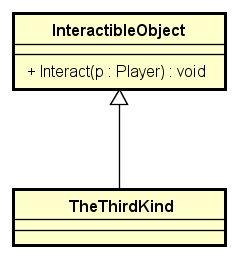
\includegraphics[scale=0.75]{diagramme/interactibleobject.png}
\caption{\lstinline{Interact} in der Klasse \lstinline{Interactible}Object und die abgeleitete Klasse \lstinline{TheThirdKind}}
\end{figure}

Das Gesprochene erscheint in einer Sprechblase. Um dies auszulösen, muss \lstinline{lastTalk} des Spielers geändert werden.
Dies passiert, wenn der Spieler mit dem \lstinline{TheThirdKind} Objekt Interagiert 
\begin{lstlisting}[caption={Setzen des Sprechinhaltes}]
void Interact(Player p)
{
	(...)
	p.lastTalk = "You must pick the two flowers and bring them to me";
	(...)
}
\end{lstlisting}

In der Funktion \lstinline{Update} des HUD wird dies dann dargestellt:
 
\begin{lstlisting}[caption={Gesprochenes aktualisieren}]
void Update()
{
	(...)
	string lastTalk = player.lastTalk;
	// wenn mit dem Spieler seit letztem Mal gesprochen wurde
	if (lastTalk.Length > 0) {
		// anzeigen der Sprechblase
		player.lastTalk = "";
		talking.SetActive(true);
		talkingText.text = lastTalk; //hier wird der Text ersetzt
		// Zeitpunkt des Anzeigens merken
		speechDisplayedTime = (int)Time.time;
	} 
}
\end{lstlisting}


\subsubsection{Autonome Gegner}
\label{subsubsec:npc}
Skript: NPC.cs\\\\
NPC bedeutet \textbf{Non-Player-Character}. Der Gegner war in der Anfangsphase der Programmierung dieses Spieles der einzige Nicht-Spieler-Character, deswegen blieb der Klassenname. Der NPC ist der Antagonist meines Spiels.
Er ist neben dem Player selber das komplizierteste Objekt.

\begin{figure}[H]
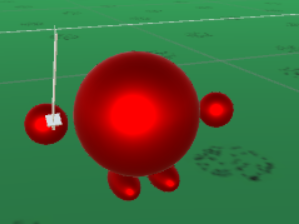
\includegraphics[scale=1]{screenshots/npc.png}
\caption{NPC 3D Modell}
\end{figure}
Das 3D Modell des NPC besteht nur aus Sphären.

\paragraph{aktivieren}
Damit der NPC auf den Spieler aufmerksam wird, muss er ihn zuerst sehen.
Dafür hat der NPC einen Collider, welcher sein Sichtfeld darstellt.
\begin{figure}[H]
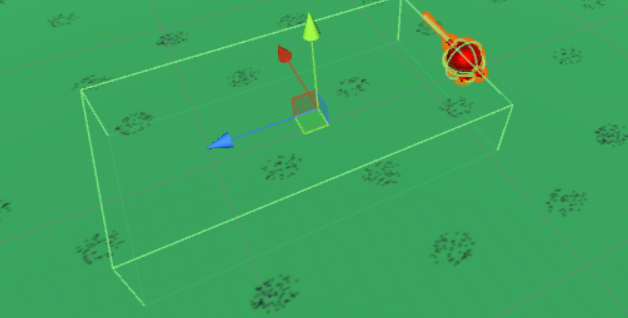
\includegraphics[scale=1]{screenshots/fov.png}
\caption{Sichtfeld des NPCs}
\end{figure}
Sobald der Spieler diesen Collider einmal ausgelöst hat, wird der Bewegungscode aktiviert.
\begin{lstlisting}
public bool hasseenplayer = false;
private void Start()
{
	player = GameObject.FindGameObjectWithTag ("Player");
}
	
//Spotting player
void OnTriggerEnter(Collider fov)
{	
	if (fov.name == "Player") {
		Debug.Log("has seen");
		hasseenplayer = true;
	}
}
\end{lstlisting}
\paragraph{bewegen }
Der NPC richtet sich nach dem Spieler aus und geht so lange auf ihn zu, bis die X und Y Koordinaten auf eine Differenz von 1 genau übereinstimmen.\footfullcite{npcmove}
Dann spielt der NPC seine Attackieren-Animation ab.
\begin{lstlisting}
if (hasseenplayer == true) {	
	// wenn Spieler in Reichweite, angreifen (fighting = true )
	Vector3 forward = transform.TransformDirection (Vector3.forward);

	
	if (Physics.Raycast (transform.position, forward, out hit, 10)) {	

		Debug.DrawLine (transform.position, hit.point);
		if (hit.collider.gameObject.tag == "Player") {
			fighting = true;
			Debug.Log("NPC is attacking");
		} else {
			fighting = false;
			anim.ResetTrigger ("Attack");
		}

		if (fighting == true) {
			// Animation Angriff starten
			anim.SetTrigger ("Attack");
			
		} else {	
			anim.SetBool ("iswalking", true);
					
			if (player.transform.position.x > (transform.position.x - 1)) {
				// Gehe nach rechts
				transform.position += new Vector3 (Speed * Time.deltaTime, 0, 0);
            		
			} else {
				// Gehe nach links
				transform.position -= new Vector3 (Speed * Time.deltaTime, 0, 0);
					}
			// Gehe zu Player's Z-Koordinate
			if (player.transform.position.z > transform.position.z) {
				// Gehe hoch
				transform.position += new Vector3 (0, 0, Speed * Time.deltaTime);
			} else {
				// Gehe runter
				transform.position -= new Vector3 (0, 0, Speed * Time.deltaTime);
			}
			transform.LookAt (target);//https://docs.unity3d.com/ScriptReference/Transform.LookAt.html
		}
	} else {
			anim.SetBool ("iswalking", false);
	}
}

\end{lstlisting}
\subsubsection{TheThirdKind.cs}
Skript: TheThirdKind.cs\\\\
\lstinline{TheThirdKind} ist ein Schlüsselelement des Spiels. Er ist ein Weiser, der den Spieler leitet. Zu ihm muss man zu Beginn gehen, um die Blumen-Aufgabe zu erhalten.
Er sollte der aus vielen RPGs bekannten Auftraggeber sein, der einen quer durch die Welt schickt um ein paar Rohstoffe zu sammeln.
\begin{figure}[H]
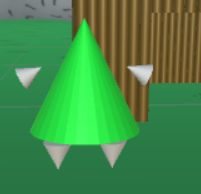
\includegraphics[scale=1]{screenshots/t3k.png}
\caption{ TheThirdKind 3D Modell}
\end{figure}
Sein 3D Modell besteht nur aus Kegeln.

\subsection{Aufgaben}

\subsubsection{Quest.cs}
Skript: Quest.cs\\\\
Eine \lstinline{Quest} ist eine einzelne Aufgabe. Sie hat einen beschreibenden Text und ein zugehöriges GameObject, das über seinen Namen festgelegt wird. Zusätzlich können Vorbedingungen in Form von zuvor zu absolvierenden Aufgaben angegeben werden.

\begin{lstlisting}
public Quest (string nameString, string taskString, Quest[] preconditions = null)
{
	name = nameString;
	task = taskString;
	done = false;
	precond = preconditions;
}
\end{lstlisting}

Eine Aufgabe kann nur dann erfüllt werden (\lstinline{CanBeDone}) wenn ihre Vorbedingungen erfüllt sind. Bei der Interaktion wird in diesem Fall die \lstinline{Done} Methode aufgerufen.

\subsubsection{Quests.cs}
Skript: Quests.cs\\\\
Diese Klasse führt die Liste aller Aufgaben, ob erledigt oder nicht. Sie  aktualisiert den HUD mit der Beschreibung der aktuellen Aufgabe und gibt bei Interaktion mit einem GameObject an, ob für dieses eine noch offene Quest \lstinline{GetActiveQuest} vorhanden ist. Aus Gründen der Einfachheit ist sie ein Attribut der \lstinline{Player} Klasse, deswegen kommunizieren die GameObjekte über die entsprechenden Methoden von \lstinline{Player}:

\begin{lstlisting}
	// Fügt der Liste eine neue Aufgabe hinzu
	public void AddQuest (Quest q)
	{
		quests.AddQuest (q);
	}

	// Sucht nach einer Aufgabe per Name
	public Quest GetQuest (string name)
	{
		return quests.GetQuest (name);
	}

	// Sucht nach einer aktiven Aufgabe per Name
	public Quest GetActiveQuest (string name)
	{
		return quests.GetActiveQuest (name);
	}
\end{lstlisting}

%\section{Feinarbeit}

%Fehlersuche

%Debug.Log

%Raycast

%Optimierung

%- 3 Arten für Referenzen zwischen Objekten

%	- IDE D und D
%	- Find by Tag
%	- Find by Name

\section{Versionsverwaltung}

Beim Klonen des Projekts auf einen Laptop stellte sich das Problem, dass das Projekt dort nicht mehr geöffnet werden konnte. Eine Suche im Forum ergab, dass Blender installiert sein muss, sonst kann das Projekt von Unity nicht geöffnet werden.\footfullcite{missingprefabs}

\section{Verteilung und Test}

\subsection{Verteilung über Github}

Da ich von Anfang an die Versionskontrolle dieser Maturaarbeit mit Github durchgeführt habe konnte sich theoretisch jeder, der meinen Github-Namen kannte, meine komplette Arbeit herunterladen.\cite{csomormaturaarbeit19github}
Ich erzählte also in der Schulklasse von meinem Projekt und einige meiner Freunde fragten, ob sie es downloaden könnten.

Leider schieden sofort einige Kandidaten aus, da sie kein Windows-Gerät besassen. Aus den restlichen drei Interessierten wurden die SimpleRPG-Beta-Tester.

\subsection{Testphase}

Diese informierten mich schon früh über Abstürze, Bugs und Unschönheiten.
An ihnen konnte ich ebenfalls die Effektivität meines \textbf{README.MD} Textes testen, welches ihnen Instruktionen für das korrekte Starten des Spiels und Informationen über die Steuerung lieferte.
Oft redeten wir in den kurzen Pausen zwischen den Lektionen über mein Spiel.
Das gab mir eine Plattform, wo ich meine weiterführenden Ideen präsentieren und sofort Feedback einholen konnte, was mir half, mich auf Inhalte zu fokussieren, die von der Mehrheit auch gemocht wurden.


